\documentclass{article}
\usepackage{tikz}
\usepackage{amsmath}

\begin{document}

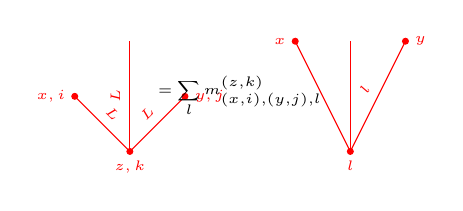
\begin{tikzpicture}[scale=0.7]
    % Left diagram
    \draw[red] (0,0) -- (1,1) node[pos=0.5, sloped, above] {\tiny$L$};
    \draw[red] (0,0) -- (-1,1) node[pos=0.5, sloped, above] {\tiny$L$};
    \draw[red] (0,0) -- (0,2) node[pos=0.5, sloped, above] {\tiny$L$};
    \filldraw[red] (0,0) circle (1.5pt) node[below] {\tiny$z,k$};
    \filldraw[red] (1,1) circle (1.5pt) node[right] {\tiny$y,j$};
    \filldraw[red] (-1,1) circle (1.5pt) node[left] {\tiny$x,i$};
    
    % Equation
    \node at (2,1) {\tiny$=\displaystyle\sum_{l} m_{(x,i),(y,j),l}^{(z,k)}$};
    
    % Right diagram
    \draw[red] (4,0) -- (5,2) node[pos=0.5, sloped, above] {\tiny$l$};
    \draw[red] (4,0) -- (3,2) node[pos=0.5, sloped, above] {};
    \draw[red] (4,0) -- (4,2) node[pos=0.5, sloped, above] {};
    \filldraw[red] (4,0) circle (1.5pt) node[below] {\tiny$l$};
    \filldraw[red] (5,2) circle (1.5pt) node[right] {\tiny$y$};
    \filldraw[red] (3,2) circle (1.5pt) node[left] {\tiny$x$};
\end{tikzpicture}

\end{document}